%\chapter{Técnicas de Visual SLAM} \label{cap:tecnicas}
\section{Técnicas de Visual SLAM} \label{s:tecnicas}

En esta sección explicaremos varios de los algoritmos conocidos hasta ahora de Visual SLAM, todos ellos se caracterizan por intentar estimar la posición de la cámara con el menor error posible junto con la generación de un mapeo del entorno que rodea a la cámara.
También se explicarán los módulos principales que componen un algoritmo de Visual SLAM.
Por último, el conjunto de algoritmos de Visual SLAM se podrían dividir en base al número de regiones que se utilizan en cada frame o imagen recibida para calcular la localización y el mapa. De un lado estarían el grupo de los algoritmos denso / escaso (\textit{dense/sparse}) \footnote{https://www.kudan.eu/kudan-news/different-types-visual-slam-systems/}, por otro lado estarían los Métodos Directos y Métodos Indirectos o basados en características que se caracterizan por el modo en el que se son procesadas las imágenes de entrada (\textit {direct/indirect}).

\subsection{Módulos del algoritmo de Visual SLAM}
La estructura de un algoritmo genérico  de Visual SLAM, podría estar dividida en varios módulos. En esta sección describiremos los 5 componentes que suelen aparecer en la mayoría de algoritmos de Visual SLAM actuales. Estos módulos podrían ser Inicialización, Localización, Generación de Mapa, Optimización global del mapa y Relocalización. Los 3 primeros módulos podrían ser considerados como básicos o esenciales para poder desarrollar correctamente el algoritmo de Visual SLAM, en cuanto a los 2 últimos no son considerados esenciales aunque sí que es muy recomendable que el sistema los tenga incorporados ya que le aportan mayor robustez y precisión al sistema. 
Los métodos de Visual SLAM utilizan diferentes metodologías para cada módulo, las características de un algoritmo Visual SLAM dependen directamente de la metodología utilizada. Por ello para conocer el rendimiento, ventajas y limitaciones de los algoritmos Visual SLAM es importante entender cada módulo del algoritmo \cite{Takafumi17}.

\begin {enumerate}
\item \textbf{Inicialización}:  Para iniciar un algoritmo de Visual SLAM es necesario definir un sistema de coordenadas que permita estimar la posición de la cámara y construir el mapa 3D inicial del entorno desconocido, normalmente mediante homografía.
\item \textbf{Localización (Tracking)}: Para la localización de la cámara es necesario realizar correspondencias 2D-3D entre la imagen captada y el mapa construido. Esto se consigue utilizando emparejamiento de puntos característicos o seguimiento de puntos en la imagen. La estimación de la  posición de la cámara se obtiene mediante el algoritmo iterativo de Gauss-Newton \footnote{https://www.youtube.com/watch?v=rpgMZRFm1aI}.
Los parámetros intrínsecos de la cámara suelen estar calibrados de antemano, por tanto son valores conocidos. Para hallar la estimación de la posición de la cámara se aplica una matriz de traslación y rotación sobre los parámetros extrínsecos de la cámara y así obtendremos las coordenadas de la cámara en el sistema global de coordenadas.
\item \textbf{Generación de Mapa}: El mapa se va generando a medida que se van añadiendo nuevas estructuras 3D de regiones que no habían sido incluidas previamente en el mapa.
\item \textbf{Optimización global}:  A medida que la cámara se va desplazando se van generando errores acumulativos de estimación de posición. Se puede calcular el error acumulativo desde el inicio hasta la posición actual cuando tras realizar varios movimientos con la cámara volvemos a visitar la imagen inicial o localización de partida. Para ello nos ayudaremos de la técnica de cierre de bucle. El cierre de bucle, es una técnica en la que se trata de encontrar la imagen actual entre las imágenes anteriormente capturadas. Si el bucle es detectado significa que la cámara ha obtenido una imagen que ya había capturado anteriormente. La técnica de cierre de bucle se realiza para obtener una geometría consistente del mapa. La técnica de \textit{Bundle Adjustment} (BA) se utiliza para minimizar el error de retroproyección del mapa mediante optimización de la posición de la cámara y del mapa.

\item \textbf{Relocalización}: Este módulo es requerido cuando falla la localización (Tracking) debido a movimientos rápidos o bruscos u oclusiones de la cámara. En este caso se debe encontrar de nuevo la posición de la cámara con respecto al mapa. Si un algoritmo de Visual SLAM no cuenta con este módulo, el sistema dejará de funcionar en caso de que se perdiese por un instante la localización de la cámara. Este módulo también es útil para resolver el problema de secuestro en robótica móvil.

\end {enumerate}



\subsection{Métodos Densos y Métodos Escasos}

Los Métodos Escasos utilizan sólo un pequeño subconjunto  de píxeles de ciertas regiones de la  imagen, mientras que los Métodos Densos utilizan la mayoría de los píxeles de la imagen captada. Por tanto los mapas generados por los Métodos Densos proporcionan muchos más detalles de la escena al utilizar muchos más puntos, pero también necesitan de una capacidad de computo muy elevada, de hecho la mayoría de Métodos Densos requieren la utilización de GPU.
Los Métodos Escasos, al tratar menos puntos, obtienen unos mapas con muy pocos detalles, más parecido a una nube de puntos, donde principalmente se representan la trayectoria y las diferentes localizaciones que ha ido ocupando la cámara en el mapa 3D.

\subsection{Métodos Directos y Métodos Indirectos}

Los Métodos Indirectos en Visual SLAM intentan extraer puntos característicos de la imagen y partiendo de estos puntos trata de calcular la posición de la cámara y de generar el mapa. Los puntos característicos pueden ser desde esquinas (obtenidas mediante algoritmo FAST) y bordes hasta otros descriptores de imagen más sofisticados como SIFT o ORB. Sin embargo, los Métodos Directos en Visual SLAM utilizan directamente los valores de intensidad de los píxeles para construir el mapa y calcular la posición de la cámara. En cuanto a los Métodos Indirectos tratan de recuperar la profundidad, estructura del entorno y la posición de la cámara a través de una optimización del mapa y los parámetros de la cámara mediante Bundle Adjustment. 

\begin{figure}[H]
\begin{center}
\subfigure[]{\label{fig:grafico}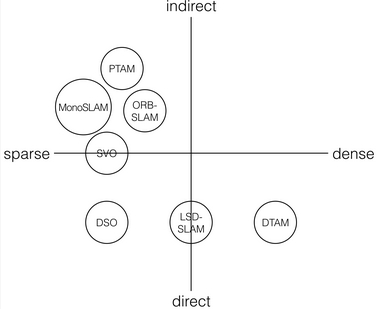
\includegraphics[height=6.0cm]{img/cap4/grafo_metodos_vslam.png}}
\end{center}
\caption{Mapa de clasificación de los principales algoritmos de Visual SLAM. }
\end{figure}
En el siguiente gráfico \ref{fig:grafico} se muestran los principales algoritmos de Visual SLAM y que posición ocuparían al clasificarlos entre Métodos Directos e Indirectos y Métodos Densos y Escasos.
Tres métodos (MonoSLAM, PTAM, ORB-SLAM ) podrían clasificarse dentro del grupo Métodos Indirectos y Escasos.
El método DSO se podría clasificar como método Escasos y Directos.
El método LSD-SLAM podrían clasificarse como un método Directo, a medio camino entre Denso y Escaso.
Como Método Denso y Directo estaría el método DTAM.
El método SVO podría clasificarse como Método Escaso pero a medias de Método Directo y Método Indirecto.
Se puede observar como la zona de Métodos Indirectos y Métodos Densos (cuadrante superior derecho) está vacía, se entiende que es por la necesidad de potencia de CPU que requerirían estos métodos, aunque no se descarta que en el futuro aparezca alǵun método en este cuadrante señalado.

%\begin{figure}[htbp]
\begin{figure}[H]
\begin{center}
\subfigure[]{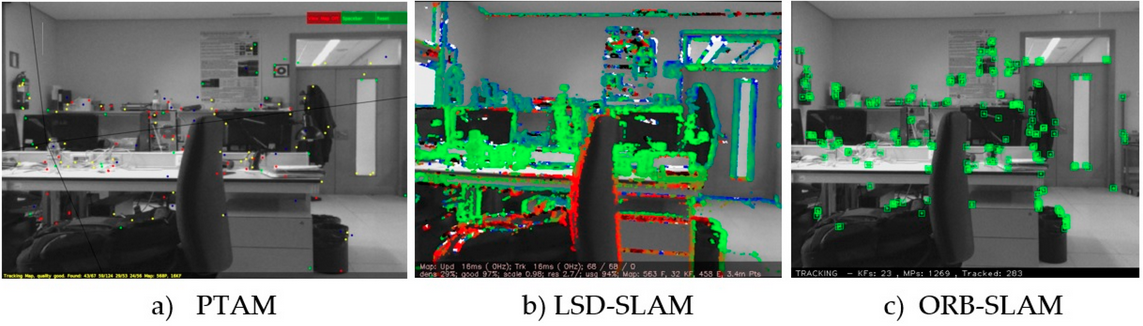
\includegraphics[height=5.0cm]{img/cap4/diferencia_Mapa_ptam-orb-lsd.png}}
\end{center}
\caption{ Diferencia entre mapas generados por distintos algoritmo de Visual SLAM (b)}
\end{figure}

\clearpage

\subsection{MonoSLAM}
El algoritmo de  MonoSLAM (\textit{Monocular SLAM}) \cite{Davison2007monoslam} utiliza solamente una cámara RGB para la localización y mapeo de entornos desconocidos. Fue desarrollado en el año 2002  por Andrew Robinson. Para estimar la posición de la cámara utiliza un filtro extendido de Kalman (EKF) y la posición de una serie de puntos 3D. Este método requiere de una inicialización con al menos 4 puntos 3D conocidos que utilizará para calcular la posición de la cámara y la generación de nuevos puntos para el mapa.
%\begin{figure}[htbp]
\begin{figure}[H]
\begin{center}
\subfigure[]{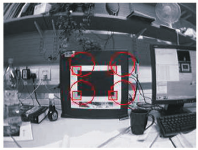
\includegraphics[height=6.0cm]{img/cap4/Initialization4PointsMonoSlam.png}}
\end{center}
\caption{Inicialización de MonoSLAM con 4 puntos conocidos.}
\end{figure}

El EKF, tiene un vector de estado compuesto de posición, orientación y velocidad de la cámara y además las coordenadas 3D de los puntos conocidos en un cierto momento, esto implica que el vector de estado irá aumentando de tamaño a medida que vayamos descubriendo nuevos puntos 3D. El modelo de observación estará compuesto de las proyecciones de cada uno de los puntos 3D en el plano imagen.

El uso de un EKF es apropiado, ya que se realizan iteraciones cada pocos milisegundos, y por tanto en intervalos de tiempo tan pequeños, el sistema puede aproximarse a un sistema lineal. Cuantas más iteraciones o frecuencia de muestreo la estimación mejora. En cada iteración se hace una detección de puntos de interés (esquinas con FAST) en la imagen actual de entrada, y obtendremos una serie de puntos que serán candidatos a ser el vector observación de los puntos que queremos seguir. Estos candidatos deberán ser filtrados, pues alguno puede ser un falsa esquina. Se utilizará una función de divergencia ZMSSD (\textit{Zero Mean Sum of Squared Differences}) entre parches para determinar si el candidato es aceptable o no. Al utilizar sólo parches de unos pocos píxeles alrededor del candidato, estamos optimizando el computo ya que no requiere procesar toda la imagen.

Aún así es posible que se acepten puntos candidatos que no sean apropiados. Para tratar de eliminar estos falsos positivos, \cite{civera20101} propuso una alternativa conocida como 1-Point RANSAC.
MonoSLAM es recomendable para mapas con pocos puntos. Es muy sensible a movimientos bruscos y por tanto difícilmente podrá recuperarse de un secuestro. Si la hipótesis de partida no es correcta el filtro podría desestabilizarse y no llegar nunca a aproximar razonablemente el vector de estado.


%\begin{figure}[htbp]
\begin{figure}[H]
\begin{center}
\subfigure[]{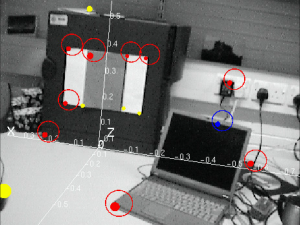
\includegraphics[height=5.0cm]{img/cap4/monoslam-300x225.png}}
\end{center}
\caption{Ejemplo de puntos característicos tomados con MonoSLAM.}
\end{figure}
\clearpage


\subsection{PTAM}
\textit{Parallel Tracking and \textit{Mapping}}. Es un algoritmo creado en 2007 por George Klein \cite{Klein2007parallel} que también calcula el Tracking y el \textit{Mapping} como en MonoSLAM pero para ello utiliza 2 \textit{Threads}, uno para calcular el posicionamiento de la cámara (Tracking ) y el segundo para la generación del mapa (\textit{Mapping}). Esta separación en dos hilos de ejecución se debe a que el Tracking necesita ser calculado en tiempo real para obtener una localización precisa, mientras que el \textit{Mapping} puede demorarse más tiempo sin perjudicar a la localización de la cámara. 

Con las imágenes captadas en secuencia se van generando \textit{Keyframes} o fotogramas clave. Se genera un nuevo \textit{Keyframe} a medida que la cámara se va desplazando. Los \textit{Keyframes} se utilizan para la localización y para ir generando el mapa de puntos.
Este algoritmo es recomendable para mapas con elevado número de puntos, es capaz de recuperarse fácilmente de un secuestro, extrae los puntos de interés mediante extracción de características como en MonoSLAM y trata de emparejarlos con los puntos extraídos de las imágenes anteriores.  Como extractor de características utiliza el detector FAST. Se realizará una subdivisión de la imagen a distintas resoluciones, normalmente 4 niveles, lo que se conoce como pirámide de la imagen y se pasará un filtro FAST sobre esta pirámide para detectar los puntos más característicos de la imagen.
Cada \textit{Keyframe} que se genera, contiene  la imagen captada junto su pirámide y sus puntos de interés detectados. Cuando añadimos un \textit{Keyframe}, se intenta localizar en este \textit{Keyframe} los puntos que ya se encuentran en el mapa, en caso de no ĺlocalizarlos se añaden nuevos puntos al mapa. Mientras no se añadan \textit{Keyframes}, se intentará mejorar el mapa con los \textit{Keyframes} disponibles optimizando con Bundle Adjustment.

Se suele utilizar en entornos cerrados y pequeños y utiliza técnicas SFM. Muy utilizado también para realidad aumentada.

%\begin{figure}[htbp]
\begin{figure}[H]
\begin{center}
\subfigure[]{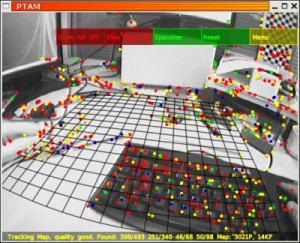
\includegraphics[height=6.0cm]{img/cap4/ptam_screenshot-300x243.jpg}}
\end{center}
\caption{Nube de puntos característicos tomados con PTAM.}
\end{figure}



\subsection{DTAM}
\textit {Dense Tracking and Mapping}. Es un método de reconstrucción de tipo denso que emplea el error fotométrico para poder trabajar en el dominio de la imagen 
\cite{Newcombe2011dtam}.

La fase de localización (Tracking) se resuelve por una formulación alternativa a EKF utilizando ESM (Minimización Eficiente de segundo orden), de esta forma se puede ejecutar en paralelo.
Para la reconstrucción del mapa emplea una metodología basada en la transformada de Radón. Cada píxel 3D será representado como un cubo, que se proyectará a cada una de las imágenes esclavas. Cuando la recta entre estos píxeles sea cero, el error fotométrico será nulo y entonces se podrá considerar que la proyección es correcta.
El algoritmo de DTAM está compuesto de los siguientes 3 componentes:
\begin{enumerate}
\item Inicialización del mapa, se realiza con medidas estéreo.

\item La posición de la cámara es estimada comparando la imagen de entrada con las imágenes sintéticas generadas por la reconstrucción del mapa.

\item La información de profundidad es estimada para cada píxel usando multi base-line estéreo y es optimizado considerando el espacio continuo.
\end{enumerate}

Para conseguir un buen rendimiento en tiempo real DTAM necesitará el uso GPU.




%\begin{figure}[htbp]
\begin{figure}[H]
\begin{center}
\subfigure[]{\label{fig:mapaDTAM}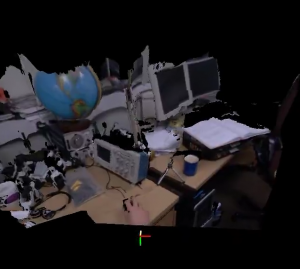
\includegraphics[height=6.0cm]{img/cap4/DTAM_taster-300x269.png}}
\end{center}
\caption{Ejemplo de mapa generado con DTAM. Todos los puntos forman parte del mapa.}
\end{figure}

\subsection{SVO}
\textit{FAST Semi-Direct Monocular Visual Odometry}.
Permite ser utilizado en ordenadores con poca potencia de computo debido a la rapidez del algoritmo.
Es un método híbrido entre los métodos de extracción de características y métodos directos
\cite{Forster2017svo}. 
Se asemeja a PTAM en que también utiliza dos \textit{Threads} independientes, el primero para Tracking y el segundo para \textit{Mapping}.
En el proceso de Tracking, el algoritmo trata de minimizar el error fotométrico, pero para acelerar el proceso sólo tiene en cuenta ciertas partes de la imagen, unos parches de 4x4 alrededor de los píxeles que se han identificado como candidatos.

Toma los puntos 3D visibles del fotograma anterior, los proyecta sobre la imagen actual, obtiene parches de dimensiones 4x4 alrededor de los píxeles y trata de hallar  el mínimo error fotométrico de esos puntos que servirá para hallar el emparejamiento entre las características de dos frames. Calcula el desplazamiento entre imágenes de forma muy eficiente.
Para la estimación del movimiento, trataremos de minimizar el error fotométrico de los parches de 4x4 anteriores.


 Como último paso haremos la minimización del error de reproyección clásica de los métodos basados en características para corregir los residuos que genere el paso anterior, los cuales podrían provocar la pérdida de ortogonalidad.
En cuanto al \textit{Mapping} utilizaremos un modelo gaussiano en torno al valor de profundidad real, cuando la incertidumbre de un parche decae, este es añadido al mapa.
Un nuevo frame tiene posibilidad de convertirse en \textit{Keyframe} si diverge lo suficiente del resto.

%\begin{figure}[htbp]
\begin{figure}[H]
\begin{center}
\subfigure[]{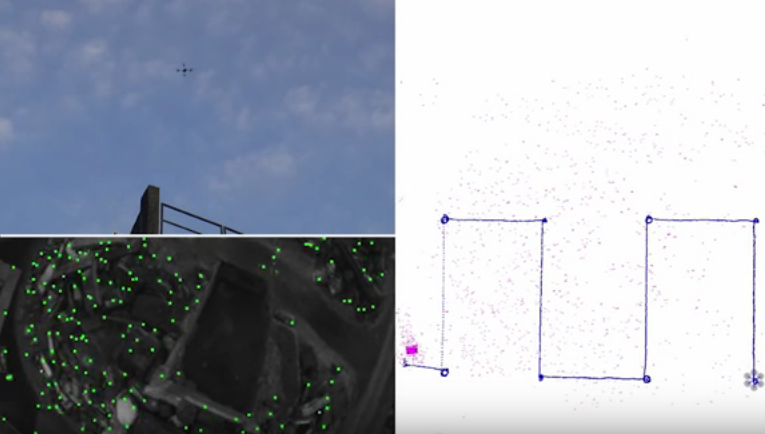
\includegraphics[height=6.0cm]{img/cap4/mapageneradoConSVO.png}}
\end{center}
\caption{Mapa generado con un dron utilizando la técnica SVO.}
\end{figure}


\subsection{LSD-SLAM} 
\textit {Large-Scale Direct Monocular SLAM}
La principal característica de este modelo es que trata de generar mapas del entorno a gran escala y consistentes.
Utiliza para ello métodos directos. A demás de tener 2 hilos como PTAM uno para Tracking y otro para \textit{Mapping}, existe un tercer componente encargado de estimar la profundidad del mapa.\cite{Engel2014lsd}
El \textit{Thread} de Tracking, parte de un \textit{Keyframe}  para calcular el desplazamiento, minimizando el error fotométrico que estará normalizado por la varianza. Utiliza una optimización ponderada de Gauss-Newton para medir la alineación entre frames.
El \textit{Thread} estimador de profundidad, inicializa el mapa de profundidad proyectando los puntos del \textit{Keyframe} anterior. Las imágenes que no son \textit{Keyframes} se usarán para refinar el \textit{Keyframe} actual. Se añadirán nuevos píxeles al mapa de profundidad cuando se encuentren zonas de la imagen con suficiente separación estéreo.
En cuanto al \textit{Thread} dedicado al proceso de \textit{Mapping}, cuenta con un mecanismo de cierre de bucle que se ejecutará cada vez que llegue un nuevo \textit{Keyframe}. En cuanto a su inicialización, solo utiliza una única imagen para generar un mapa inicial de profundidad que irá convergiendo hacia unos valores de profundidad correctos a medida que la cámara se vaya desplazando.
Este método es capaz de funcionar en tiempo real en un PC, pero  no funciona muy bien en dispositivos con limitada potencia de CPU.

%\begin{figure}[htbp]
\begin{figure}[H]
\begin{center}
\subfigure[]{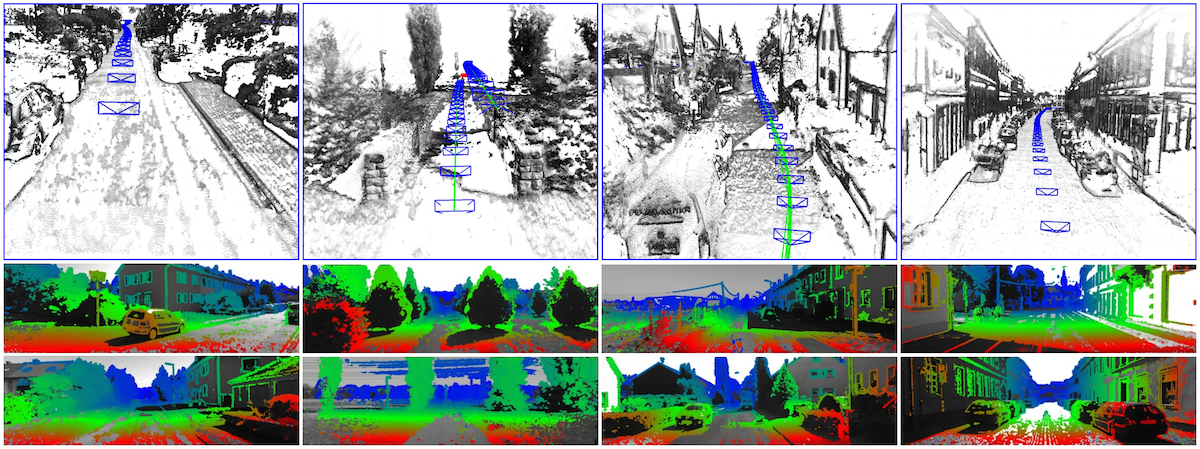
\includegraphics[height=6.0cm]{img/cap4/stereo-lsd-slam.png}}
\end{center}
\caption{Mapa generado con LSD-SLAM y cámara estéreo}
\end{figure}

\clearpage

\subsection{ORB-SLAM}
Es un algoritmo basado en extracción y emparejamiento de píxeles característicos mediante descriptores ORB, estos descriptores son más fiables que los parches tradicionales y por tanto permiten obtener mapas robustos y precisos tanto en escenarios de grandes dimensiones como en zonas pequeñas, sin embargo para su funcionamiento en tiempo real requiere la utilización de ordenadores con alta capacidad de proceso \cite{Mur2015orb}.
Puede ser utilizado con una cámara o dos e incluso con cámaras de profundidad RGBD. Para cierres de bucle y relocalización utiliza un modelo de bolsa de palabras \cite{galvez2012bags}.
Utiliza 3 \textit{Threads}, el primero para Tracking, el segundo para \textit{Mapping} y un tercero para detectar cierres de bucle. 

En el proceso de Tracking, se trata de calcular la posición actual a partir de los emparejamientos encontrados de los puntos 3D en el fotograma anterior, para ello utilizará los descriptores ORB.
En caso de perdida, el robot podrá relocalizarse gracias a un modelo de bolsa de palabras que le permitirá encontrar \textit{Keyframes} candidatos que concuerden con la observación actual (Figura \ref{fig:ORBMatching}).

En el proceso de \textit{Mapping}, se inicializarán 2 mapas, uno por homografía y el segundo mediante una matriz fundamental. Los 2 mapas recibirán una puntuación y se elegirá como candidato para inicializar el mapa aquel que obtenga mayor puntuación. Cuando ya se dispone del mapa inicial, se procesan los \textit{Keyframes} creando nuevos puntos 3D y se optimiza localmente el mapa mediante Bundle Adjustment. A su vez se genera un grafo donde cada \textit{Keyframe} se corresponde con un vértice y un vértice estará unido a otro siempre y cuando los \textit{Keyframe} tengan varios puntos 3D en común. Este grafo permite la eliminación de \textit{Keyframe} redundantes (Figura \ref{fig:ORB_SLAM}).

En el proceso de Looping, se comprobará si se ha producido un cierre de bucle. Utilizando el grafo de \textit{Keyframe} conectados y el modelo de bolsa de palabras se intenta encontrar \textit{Keyframe} candidatos que tengan una apariencia similar a la imagen actual.

%\begin{figure}[htbp]
\begin{figure}[H]
\begin{center}
\subfigure[]{\label{fig:ORBMatching}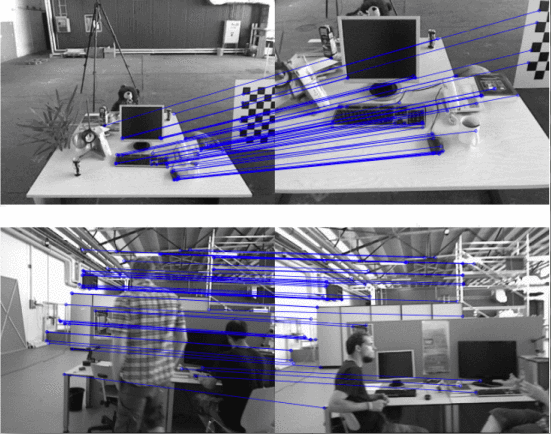
\includegraphics[height=5.5cm]{img/cap4/ORB_localization.png}}
\hspace{0.5cm}
\subfigure[]{\label{fig:ORB_SLAM}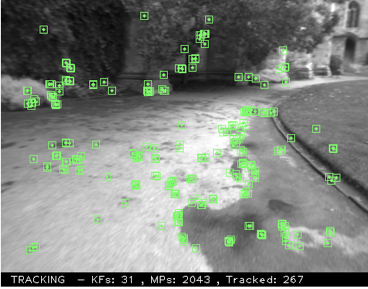
\includegraphics[height=5.5cm]{img/cap4/ORB_SLAM.png}}
\end{center}
\caption{Localización de puntos característicos en 2 imágenes con ORB }
\end{figure}

\clearpage

\subsection{DSO}
\textit{Direct Sparse Model}.
Está basado en optimizaciones continuas del error fotométrico sobre una ventana de frames recientes\cite{Engel2016direct}.
El inicio del Tracking, cuando se crea un nuevo \textit{Keyframe}, todos los puntos activos son proyectados en el y ligeramente dilatados, creando así un mapa de profundidad semi denso. Nuevos frames son creados con respecto a este frame utilizando alineamiento directo de 2 frames, una pirámide multi escala y un modelo de movimiento constante a inicializar. 
Para la relocalización, se podrán trazar hasta 27 rotaciones pequeñas en diferentes direcciones. Esta recuperación de posición se consigue en el nivel más pequeño de la pirámide de la imagen.
La creación de \textit{Keyframes} es similar a ORB-SLAM, existen 3 criterios para determinar cuando se necesita un nuevo \textit{Keyframe}.
\begin {enumerate}
\item Se creará un nuevo \textit{Keyframe} (Figura \ref{fig:mapaDSO}) cuando la imagen de entrada cambie notablemente con respecto al último \textit{Keyframe}, esto se medirá con la diferencias de medias al cuadrado entre los píxeles.
\item La traslación de la cámara causa oclusiones y des-oclusiones, lo cual indica que se deben generar nuevos \textit{Keyframes}
\item Si el tiempo de exposición de la cámara cambia significativamente, se deberá tomar un nuevo \textit{Keyframe}. Esto se mide por el factor de brillo relativo entre 2 frames. 
\end {enumerate}

En cuanto al rechazo de \textit{Keyframes}, sigue la siguiente estrategia. Sean $I_1$ \dots $I_n$ un conjunto de \textit{Keyframes} activos, siendo $I_1$ el más nuevo y $I_n$ el más antiguo
\begin {enumerate}
\item Siempre se mantendrán los dos últimos \textit{Keyframes} ($I_1$  e $I_2$ )
\item Frames con menos del 5\% de sus puntos visibles en $I_1$  son descartados.
\item Si mas de N frames están activos, se descartan (exceptuando $I_1$  e $I_2$) aquel que maximice un marcador de distancia d(i,j) donde d(i,j) es la distancia Euclídea entre \textit{Keyframes} $I_1$  e $I_j$
\end {enumerate}

Sobre el tratamiento de los puntos, siempre se tratará de mantener un numero fijo de puntos activos repartidos de forma uniforme entre el espacio y los frames activos. En un primer paso, se identifican Np puntos candidatos en cada nuevo \textit{Keyframe}. Los puntos candidatos no son inmediatamente sumados a la optimización, sino que son localizados individualmente en sucesivos frames generando una primera estimación del valor de profundidad que servirá como inicialización. 

En cuanto a la selección de puntos candidatos, se intentará seleccionar aquellos puntos que están bien distribuidos en la imagen y tienen un valor elevado de gradiente con respecto a sus alrededores. Para obtener una distribución uniforme de puntos sobre la imagen, esta se divide en bloques de $dxd$, de cada bloque se elegirá el píxel con el mayor gradiente siempre y cuando supere un umbral, de lo contrario no se selecciona el píxel de ese bloque. Los puntos candidatos son localizados en siguientes frames utilizando una búsqueda sobre la línea epipolar minimizando el error fotométrico. Una vez hallamos encontrado las coincidencias preparamos un valor de profundidad y la varianza asociada que se utilizará para restringir el intervalo de búsqueda en frames siguientes. Esta estrategia de localización está inspirada en LSD-SLAM.

Por último, la activación de puntos candidatos, cuando un conjunto de puntos antiguos son marginados, nuevos puntos candidatos son activados para remplazarlos, siempre intentando mantener una distribución uniforme de puntos por toda la imagen \footnote{https://ieeexplore.ieee.org/stamp/stamp.jsp?arnumber=7898369}.

%\begin{figure}[htbp]
\begin{figure}[H]
\begin{center}
\subfigure[]{\label{fig:mapaDSO}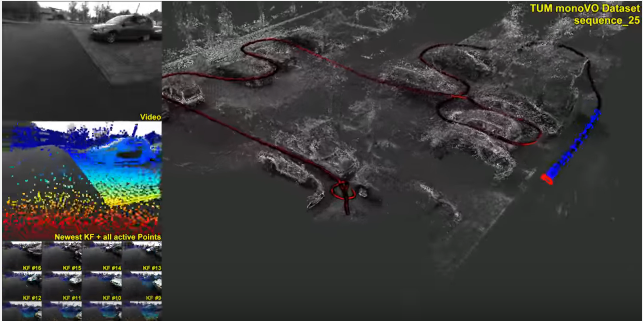
\includegraphics[height=6.0cm]{img/cap4/mapaDSO.png}}
\hspace{0.5cm}
\subfigure[]{\label{fig:fotogramaDSO}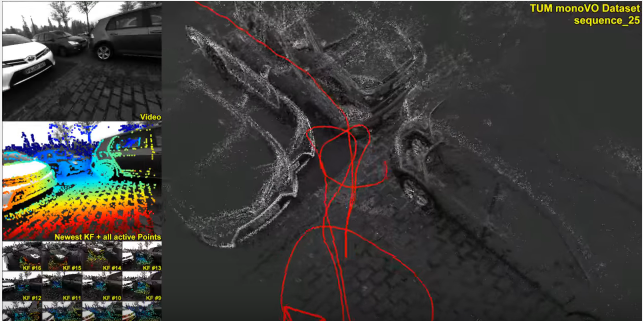
\includegraphics[height=6.0cm]{img/cap4/fotogramaDSO.png}}
\end{center}
\caption{Mapa generado con DSO (a) Ligero error en la posición al volver al punto de partida (b).}
\end{figure}

\clearpage

\subsection{SDVL}
\textit{Semi-Direct Visual Localization}. Al igual que PTAM este método tiene 2 \textit{Threads} .
El primer \textit{Thread} se utiliza para Tracking. Calcula el desplazamiento de la cámara entre dos observaciones utilizando el mapa 3D y las imágenes capturadas. Al ser un método híbrido, calculará los desplazamientos basándose en técnicas de métodos directos y píxeles característicos. El sistema cuenta también con un sistema de rechazo de espurios que ayudará a identificar y eliminar puntos 3D mal posicionados \cite{Perdices17}.
El segundo \textit{Thread} se utiliza para el \textit{Mapping}.  Se encarga de crear y actualizar el mapa del entorno del robot. Almacenará P puntos 3D  en varias imágenes desde las que se pueden observar los P puntos 3D. Sólo pasarán a ser parte del mapa aquellos fotogramas que cumplan ciertos requisitos, aquellos que sean considerados fotogramas clave o \textit{Keyframes}.
El mapa inicial se obtiene por Homografía. Es un método capaz de manejar miles de puntos en el mapa, aunque no es considerado un mapa denso, por lo que el mapa generado no contiene muchos detalles y no es capaz tampoco de generar mapas grandes. En caso de perdida de la posición de la cámara, es capaz de realizar relocalización aunque no es capaz de detectar bucle cerrado.


\subsection{RGB-D Visual SLAM}
Las cámaras RGB-D, utilizadas en dispositivos como Kinect o smartphones en el Proyecto Tango, son capaces de proporcionar información 3D del entorno en tiempo real y por tanto estas cámaras también son utilizadas en Visual SLAM.

A diferencia con los algoritmos del tipo monocular VisualSLAM, la escala del sistema de coordenadas es conocida para las cámaras RGB-D ya que son capaces de obtener las medidas y dimensiones de los objetos en 3D del entorno que le rodea.
Para estimar el movimiento de la cámara se utiliza el algoritmo ICP \textit{Iterative Closest Point}.
La mayoría de cámaras que son capaces de medir la profundidad de los píxeles están creadas para entornos cerrados o de pequeñas dimensiones. Esto es debido a que estas cámaras proyectan un patrón de infrarrojos para medir la profundidad del entorno y es difícil detectar el patrón de infrarrojos emitidos en el exterior ya que la propia luz solar generaría ruido o perturbaciones en el rango infrarrojo. Además el rango de profundidad de pueden captar los sensores RGB-D está limitado de 7 a 9 metros.
Para la localización, el movimiento relativo de la cámara es estimado identificando la localización de varios puntos característicos entre frames sucesivos. Utilizando estos puntos característicos se hace la estimación de los valores de una matriz de traslación. Con el algoritmo ICP y mapas de profundidad podremos optimizar esta matriz de traslación. También se utilizan métodos de localización basados en consistencia fotométrica similar a las técnicas utilizada en los métodos densos de Visual SLAM \cite{Takafumi17}.

Para obtener un mapa geométricamente consistente, se utilizan varios algoritmos de optimización como pose-graph y deformation-graph.
Pose-graph se utiliza para reducir el error acumulativo. Pose-graph es muy similar al bucle cerrado en los algoritmos de monocular VisualSLAM.
En contraste con otros algoritmos, la estimación de mapa también está refinada. La optimización por Deformation Graph es muy utilizada para ciertos frames y la localización de la cámara es estimada con emparejamientos entre las imágenes RGB-D y el modelo reconstruido.
Las APIs para RGB-D SLAM vienen incorporadas en dispositivos como Google Tango y Structure Sensor. Especialmente, Google Tango proporciona una estimación de resultado estable combinando también la información proporcionada por otros sensores internos del dispositivo.

\subsection{Comparativa de los algoritmos más representativos} 
A continuación se presenta una tabla que muestra las características principales de cada algoritmo. Esta tabla es similar a la que aparece en \cite{Perdices17} pero en este caso se ha añadido el algoritmo DSO.

\begin{center}
% \begin{tabular}{||c c c c c c c c||} 
\begin{tabular}{ |m{2.5cm} | m {1.5cm}| m {1.7cm}| m {1.7cm} | m {1.7cm}| m {1.7cm}| m {1.7cm}| m {1.7cm}| }
 \hline
 Funcionalidad & Mono-SLAM & PTAM & SVO & LSD-SLAM & ORB-SLAM & SDVL & DSO  \\ [0.5ex] 
 \hline\hline
 Probabilístico & Sí & No & No & No & No & No & No \\ 
 \hline
 Hilos de ejecución & 1 & 2 & 2 & 3 & 3 & 2 & 2\\
 \hline
 Emparejamien-to & Parches & Parches & Híbrido &  Métodos directos & ORB & Híbrido & Métodos directos \\
 \hline
 Puntos 3D con incertidumbre & No & No & Sí & Sí & No & Sí & Sí\\
 \hline
 Mapa inicial & Dado & Homograf. & Homograf. & Incerti-dumbre & Homog. /Matriz F. & Homograf. & Incerti-dumbre \\ [1ex] 
 \hline
 \textit{Keyframes} & No & Sí & Sí & Sí & Sí & Sí & Sí  \\ [1ex] 
 \hline
 Puntos en mapa & Cientos & Miles & Miles & Miles & Miles & Miles & Miles \\ [1ex] 
 \hline
 Mapa denso & No & No & No & Sí & No & No & Semi-denso\\ [1ex] 
 \hline
 Gestión de mapas grandes & No & No & No & Sí & Sí & No & Sí \\ [1ex] 
 \hline
 Relocalización & No & Sí & Sí & Sí & Sí & Sí & No\\ [1ex] 
 \hline
 Rechazos de espurios & No & No & No & Sí & Sí & Sí & No\\ [1ex] 
 \hline
 Cierre de bucle & No & No & No & Sí & Sí & No & Sí\\ [1ex] 
 \hline
\end{tabular}
\end{center}


